% \documentclass[pdflatex,11pt]{aghdpl}
\documentclass{aghdpl}               % przy kompilacji programem latex
% \documentclass[pdflatex,en]{aghdpl}  % praca w j�zyku angielskim
\usepackage[polish]{babel}
\usepackage[latin2]{inputenc}

% dodatkowe pakiety
\usepackage{enumerate}
\usepackage{listings}
\lstloadlanguages{TeX}

%---------------------------------------------------------------------------

\author{Marta Ry�ko, Anna Skiba}
\shortauthor{M. Ry�ko, A. Skiba}

\titlePL{R�wnoleg�e algorytmy optymalizacji toru przejazdu w narciarstwie alpejskim}
\titleEN{Parallel algorithms for ski-line optimisation in alpine ski racing}

\shorttitlePL{R�wnoleg�e algorytmy optymalizacji toru przejazdu w narciarstwie alpejskim} % skr�cona wersja tytu�u je�li jest bardzo d�ugi
\shorttitleEN{Parallel algorithms for ski-line optimisation in alpine ski racing}

\thesistypePL{Praca magisterska}
\thesistypeEN{Master of Science Thesis}

\supervisorPL{dr in�. Roman D�bski}
\supervisorEN{Roman D�bski Ph.D}

\date{2013}

\departmentPL{Katedra Informatyki}
\departmentEN{Department of Computer Science}

\facultyPL{Wydzia� Informatyki, Elektroniki i Telekomunikacji}
\facultyEN{Faculty of Computer Science, Electronics and Telecommunication}

\acknowledgements{Serdecznie dzi�kuj� \dots}



\setlength{\cftsecnumwidth}{10mm}

%---------------------------------------------------------------------------

\begin{document}

\titlepages

\tableofcontents
\clearpage

\chapter{Wst�p}
\label{cha:wstep}

W zawodowym sporcie, trening wspomagany jest od dawna komputerami. Symulacje, analiza i por�wnywanie sekwencji ruch�w, modelowanie sylwetki w celu minimalizacji opor�w ruchu, s� metodami, kt�rymi pos�uguj� si� trenerzy w wielu dyscyplinach sportu. Narciarstwo nie jest wyj�tkiem. Istniej� zaawansowane programy pozwalaj�ce analizowa� nagrania wideo z trening�w. Nie ma jednak narz�dzia, kt�re pozwoli�o by znale�� optymalny, tj. najszybszy poprawny tor przejazdu uwzgl�dniaj�cy narzucone ograniczenia.

Znajdowane toru pretenduj�cego do bycia nazwanym optymalnym, szczeg�lnie dla d�u�szych tras, jest problemem z�o�onym obliczeniowo. Spr�bujmy wyobrazi� sobie realne zastosowanie, w kt�rym trener czy te� zawodnik, tu� przed zawodami czy treningiem, najpierw mapuje faktyczne rozstawienie bramek slalomowych za pomoc� aplikacji mobilnej zainstalowanej na urz�dzeniu z bardzo dok�adnym odbiornikiem sygna�u GPS, a nast�pnie chce w czasie prawie rzeczywistym otrzyma� odpowied� - tj. jak najlepszy tor, kt�ry powinien zosta� wybrany podczas przejazdu. Ze wzgl�du na wymagan� szybko�� odpowiedzi, obliczenia nie mog� by� wykonywane na samym urz�dzeniu mobilnym. Interesuj�cym rozwi�zaniem jest u�ycie do tego celu nie tyle p�atnych serwer�w w chmurze, co wykorzystanie mocy obliczeniowej drzemi�cej w maszynach innych fan�w narciarstwa w modelu Volunteer Computing.

Narciarstwo alpejskie to dyscyplina z d�ug� histori�. Rozw�j sportowej wersji narciarstwa alpejskiego rozpocz�� si� w po�owie XIX wieku, jednak nadal nie ma i prawdopodobnie nigdy nie b�dzie naukowej formu�y opisuj�cej tor po jakim nale�y si� porusza�, aby zadan� tras� przejecha� najszybciej. Ogromna ilo�� czynnik�w, kt�re wp�ywaj� na czas przejazdu znacznie utrudnia jej znalezienie. W sportowych dyscyplinach narciarstwa alpejskiego celem jest przejechanie w jak najkr�tszym czasie wyznaczonej trasy od startu do mety, przeje�d�aj�c przez wszystkie ustawione na trasie bramki - wymuszaj�ce skr�ty.

Problem, jakiego rozwi�zania podejmujemy si� w pracy, to problem optymalizacyjny rozwi�zywany za pomoc� symulacji komputerowej. Problem dotyczy znalezienia optymalnego toru przejazdu narciarza po trasie slalomu, kt�ry nak�ada ograniczenia na ten tor w postaci bramek. Ka�da bramka �ci�le narzuca, z kt�rej strony nale�y j� przejecha�, a omini�cie chocia� jednej z nich powoduje dyskwalifikacj� zawodnika.

Zdefiniowany przez nas problem jest interdyscyplinarny - z pogranicza fizyki i informatyki. Do dobrego zrozumienia zjawisk zachodz�cych na stoku narciarskim cenne jest te� posiadanie w�asnych do�wiadcze� z jazdy po trasach slalomu. Wymagania te powoduj�, �e problem nie jest trywialny do rozwi�zania i w celu badania go nieod��czne s� osoby o r�nych kompetencjach.

Obecnie nie uda�o nam si� znale�� publicznie dost�pnych prac, kt�re podchodzi�yby do rozwi�zania tego praktycznego problemu. Zdajemy sobie spraw�, �e problem jest bardzo z�o�ony i pr�by jego rozwi�zania to tak naprawd� poszukiwanie rozwi�zania uproszczonego tego problemu. Dodatkowo, uwzgl�dni� trzeba fakt, �e wiele zmiennych wyst�puj�cych w r�wnaniach wp�ywa na siebie nawzajem, powoduj�c zmiany niekoniecznie widoczne natychmiast. Mo�e to na przyk�ad sprawia�, �e niewielka zmiana dokonana na pocz�tku jazdy mo�e mie� znacz�cy wp�yw na ostateczny wynik, co znacznie utrudnia wszelk� predykcj� na temat wp�ywu zmian.
Aby rozwi�za� problem, stworzy�y�my fizyczny model narciarza - zamodelowany jako punkt materialny o konfigurowalnych parametrach, co umo�liwia por�wnanie wynik�w np. dla zawodnik�w o r�nych masach. Potraktowanie narciarza jako punktu materialnego jest pierwszym z zastosowanych uproszcze�, kt�re zdecydowa�y�my si� przyj�� w naszym rozwi�zaniu. Stok modelowany jest jako p�aszczyzna o zadanym k�cie nachylenia, na kt�rej za pomoc� wsp�rz�dnych oznaczamy miejsce wyst�powania bramek. Du�ym wyzwaniem by�o dobranie przybli�enia trasy przejazdu, aby umo�liwi� wystarczaj�co �atwe obliczenia i jednocze�nie nie trac�c zbytnio na dok�adno�ci oddania realnej trasy. �amana, kt�r� wybra�y�my jako rozwi�zanie spe�niaj�ce obydwa te wymagania, jest wystarczaj�co dobrym przybli�eniem je�li narzucimy na ni� dodatkowe ograniczenia jak eliminacja ostrych k�t�w za�amania.

Kluczow� cz�ci� naszego rozwi�zania jest wykorzystanie algorytmu genetycznego do wybrania pewnego lokalnego optimum trasy, a nast�pnie przeprowadzenie lokalnej optymalizacji celem wyg�adzenia znalezionego rozwi�zania. Aby przyspieszy� obliczenia, zastosowa�y�my architektur� opart� o rozproszonych klient�w wykonuj�cych obliczenia i raportuj�cych do g��wnego serwera. Na podstawie zebranych danych od klient�w, serwer jest w stanie dostarczy� rozwi�zanie szybciej oraz mo�na mie� wi�ksz� pewno��, i� jest ono, je�li nie optymalne, to bardzo bliskie optymalnego. Obliczenia wykonywane s� w �rodowisku przegl�darek internetowych w j�zyku JavaScript w modelu Volunteer Computing.

Otrzymane rozwi�zanie mo�e mie� zastosowanie nie tylko w celu znajdowania optymalnej trasy przejazdu po zadanym slalomie. Przyk�adem mo�e by� wsparcie dla trener�w ustawiaj�cych takie slalomy w postaci aplikacji podpowiadaj�cej gdzie ustawi� kolejn� bramk�, aby nie by�o problem�w z jej przejechaniem. Dodatkowo, dok�adaj�c modu� wyliczaj�cy napr�enia i si�y dzia�aj�ce na stawy kolanowe, mo�na by zredukowa� negatywny wp�yw niefortunnie ustawionych bramek, powoduj�cych wyj�tkowe przeci��enia w kolanach, wykrywaj�c to i przestawiaj�c bramki.

%---------------------------------------------------------------------------

\section{Cele pracy}
\label{sec:celePracy}

Celem poni�szej pracy jest zapoznanie student�w z systemem \LaTeX~w zakresie umo�liwiaj�cym im samodzielne, profesjonalne z�o�enie pracy dyplomowej w systemie \LaTeX.


%---------------------------------------------------------------------------

\section{Zawarto�� pracy}
\label{sec:zawartoscPracy}

W rodziale~\ref{cha:pierwszyDokument} przedstawiono podstawowe informacje dotycz�ce struktury dokument�w w \LaTeX u. Alvis~\cite{Alvis2011} jest j�zykiem 



















\chapter{Wprowadzenie teoretyczne}
\label{cha:wstepTeoretyczny}

Zrozumienie istoty przedstawionego w tej pracy rozwi�zania doboru optymalnej trasy narciarza, zar�wno pod wzgl�dem algorytmicznym jak i architektonicznym, wymaga zaznajomienia si� z istotnymi poj�ciami. W tym rozdziale, przedstawimy i opiszemy te poj�cia.

\section{Jazda po zadanym torze w narciarstwie alpejskim}
\label{sec:alpineSkiing}

Sportowa jazda na nartach zjazdowych podzielona jest na kilka dyscyplin. S� to: slalom (SL), slalom gigant (GS), super gigant (GS) oraz zjazd (DH). Elementem wsp�lnym ka�dej z nich jest konieczno�� pokonania trasy, od startu do mety, w jak najkr�tszym czasie i przy prawid�owym przejechaniu ka�dej z bramek znajduj�cych si� na trasie przejazdu. Szczeg�owe zasady dotycz�ce parametr�w stoku i sprz�tu okre�la regulamin organizacji FIS (Federation International du Ski), z po�r�d kt�rych najbardziej istotnymi s�:

\begin{itemize}
\item minimalna i maksymalna r�nica wzniesie� na trasie
\item minimalna i maksymalna odleg�o�� pomi�dzy kolejnymi bramkami
\item ilo�� bramek jaka powinna si� znale�� na trasie - proporcjonalnie do r�nicy wzniesie�
\item wymagana d�ugo�� narty
\item wymagany promie� skr�tu narty
\end{itemize}

Parametry te r�ni� si� w zale�no�ci od dyscypliny. Najbardziej techniczn� dyscyplin� jest slalom, nazywany wcze�niej slalomem specjalnym. Techniczno�� tej dyscypliny polega na du�ej ilo�ci bramek znajduj�cych si� w niewielkiej odleg�o�ci od siebie, co wymusza cz�ste skr�ty. Zawodnicy je�d�� slalom na nartach o bardzo ma�ym promieniu skr�tu, rz�du 11 metr�w. Bramka w slalomie sk�ada si� z dw�ch tyczek tego samego koloru. W slalomie gigancie, odleg�o�ci mi�dzy kolejnymi bramkami s� wi�ksze, co implikuje szybsz� jazd�. Bramka w tej dyscyplinie sk�ada si� z czterech tyczek tego samego koloru, po dwie na ka�dy koniec bramki. Dodatkowo ka�de dwie tyczki z ko�ca bramki po��czone s� p�acht� tego samego koloru co tyczki - czerwon� lub niebiesk�. Zawodnicy do tej dyscypliny u�ywaj� nart o promieniu nawet 30 metr�w. Kolejne dyscypliny s� jeszcze szybsze a promienie nart coraz wi�ksze. Bramki zar�wno w super gigancie jak i zje�dzie, s� analogiczne do tych gigantowych, r�ni� si� tylko szeroko�ci� p�acht. Super gigant, to bardziej \quotedblbase wypuszczony\textquotedblright slalom gigant, czyli slalom na kt�rym odleg�o�ci mi�dzy bramkami s� ju� bardzo du�e, a pr�dko�� proporcjonalnie ro�nie. Zjazd to ju� typowa dyscyplina szybko�ciowa. Na trasie zakr�ty wynikaj� prawie tylko z konfiguracji terenu. Dodatkowo zdarzaj� si� na trasie elementy ukszta�towania terenu na kt�rych zawodnicy wybijaj� si� i skacz� po nawet 20 metr�w.

Aby poprawnie przejecha� przez bramk� na trasie, w ka�dej z opisywanych wy�ej dyscyplin, nale�y przejecha� pomi�dzy tyczkami wyznaczaj�cymi tzw. \textit{�wiat�o bramki}. Bramki wymuszaj� skr�ty, ale nie jest tak, �e ustawione s� zawsze rytmicznie tzn. wymuszaj�c skr�ty raz w praw�, raz w lew� stron� o tym samym promieniu. Najcz�ciej spotykanym rodzajem bramki jest tzw. \textit{bramka otwarta}. Bramka otwarta, charakteryzuje si� tym, �e �wiat�o bramki znajduje si� prostopadle do linii spadku stoku. Poza bramkami otwartymi, bramki mog� by� ustawione w tzw. figury slalomowe. Pierwsz� z nich jest \textit{przelot} i mo�e wyst�powa� w ka�dej z dyscyplin. Przelot polega na ustawieniu dw�ch kolejnych bramek w taki spos�b, �e nie wymuszaj� skr�tu pomi�dzy nimi. Przelot stosowany jest w celu adaptacji trasy przejazdu do konfiguracji terenu, np. gdy na trasie naturalnie wyst�puje d�u�szy skr�t w jedn� ze stron lub rozp�dzeniu narciarza. Kolejn� figur�, stosowan� ju� tylko w slalomie, jest \textit{�okie�}. �okie� to dwie bramki ustawione w bliskiej odleg�o�ci jedna pod drug� w linii spadku stoku. S� to bramki zamkni�te, czyli �wiat�o bramki jest zgodne z lini� spadku stoku. Figura ta wprowadza zmian� rytmu i r�wnie� pozwala na dostosowanie trasy do konfiguracji terenu. Ostatni� z figur, r�wnie� stosowan� tylko w slalomie, jest \textit{wertikal}. Wertikal to bramki ustawione tak samo jak w przypadku �okcia, czyli jedna pod drug�, w linii spadku stoku, z tym, �e zamiast dw�ch, mo�e by� trzy, cztery czy nawet pi�� kolejno tak ustawianych bramek.

%TODO FIXME Marta - napisz �e czasem warto zrobi� wcze�nie skr�t a czasem nie i o podkr�conych bramkach
Opisanie wy�ej wymienionych element�w, by�o istotne by zrozumie� problem znajdowania optymalnej trasy. Najtrudniejsze jest bowiem optymalne przejechanie figur slalomowych. Podczas ogl�dania trasy, przed zawodami czy te� podczas trening�w, zawodnicy zwracaj� du�� uwag� na zapami�tanie wyst�puj�cych po sobie figur i przewidywanie, na podstawie do�wiadczenia, w jaki spos�b nale�y najecha� na dan� figur�, by zmie�ci� si�, czy te� najszybciej pokona� kolejne, nast�puj�ce po danej figurze bramki. Poprzez najazd na figur�, rozumiemy moment rozpocz�cia i spos�b prowadzenia skr�tu przed figur�. Im wcze�niej narciarz zrobi najazd, tym szybciej, po poprawnym przejechaniu bramki, b�dzie m�g� zmieni� kierunek jazdy do kolejnych tyczek.

%---------------------------------------------------------------------------

\section{Fizyczny model narciarza}
\label{sec:fizycznyModel}

%TODO FIXME jedno zdanie na temat rozdzia�u?

\subsubsection{Si�a oporu powietrza}
\label{sec:oporPowietrza}
Si�a oporu powietrza jest przyk�adem si�y tarcia p�ynu. Zale�no�� warto�ci tej si�y od pr�dko�ci mo�e by� bardzo z�o�ona i skomplikowana i tylko w specjalnych przypadkach mo�e by� rozwi�zana analitycznie. Dla bardzo ma�ych warto�ci pr�dko�ci, dla ma�ych cz�stek, si�a oporu powietrza jest wprost proporcjonalna do pr�dko�ci, a zale�no�� ta mo�e by� opisana r�wnaniem:

\begin{equation}
F_d = v b
\end{equation}

v - pr�dko�� narciarza

Dla wi�kszych pr�dko�ci i wi�kszych obiekt�w, si�a oporu powietrza jest w dobrym przybli�eniu proporcjonalna do kwadratu pr�dko�ci i zale�no�� t�, mo�na opisa� r�wnaniem:


\begin{equation}
F_d = \frac{1}{2}C\rho Av^2
\end{equation}

C - wsp�czynnik oporu powietrza, typowe warto�ci oscyluj� mi�dzy 0.4 a 1

$\rho$ - g�sto�� powietrza w jednostce $\frac{kg}{m^3}$. Warto�ci g�sto�ci powietrza przy przeci�tnym ci�nieniu wahaj� si� mi�dzy 1.26 a 1.42 w zale�no�ci od temperatury.

A - frontalna powierzchnia narciarza w projekcji prostopad�ej do wektora pr�dko�ci narciarza wyra�ona w $m^{2}$.

\begin{figure}[h]
\centering
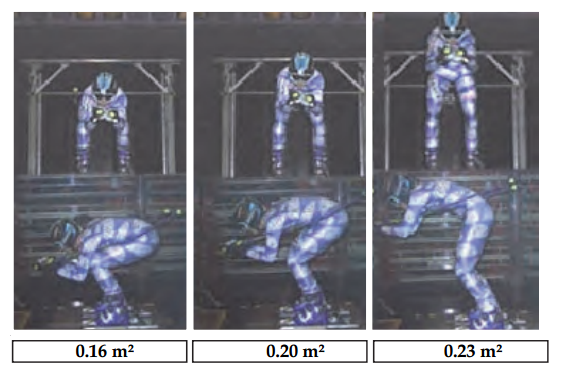
\includegraphics{airDrag}
\end{figure}

%TODO biblio link do badan
Na grafice widzimy warto�� wsp�czynnika $A$ w zale�no�ci od pozycji narciarza. Grafika pochodzi z bada� prowadzonych w tunelu aerodynamicznym IAT we Francji, przez Caroline Barelle z National Technical University of Athens z Grecji.

Pozycja narciarza ma znacz�cy wp�yw na warto�� wsp�czynnika $A$. Przyj�cie pozycji zjazdowej redukuje w stosunku do pozycji podniesionej, warto�� wsp�czynnika nawet o jedn� trzeci�. Warto nadmieni� r�wnie�, �e narciarze, nawet na amatorskich zawodach ubrani s� w specjalne kombinezony tzw. \textit{gumy narciarskie}. Kombinezony te s� jednocz�ciowe i �ci�le przylegaj� do cia�a. Nie posiadaj� �adnych odstaj�cych element�w, czasami zawieraj� tylko wewn�trzne ochraniacze w miejscach w kt�rych narciarz uderza przy ka�dym skr�cie cia�em w tyczk�. Powodem dla kt�rego str�j ten jest tak popularny r�wnie� w amatorskim sporcie jest fakt, �e znacz�co zmniejsza op�r powietrza, w stosunku do klasycznego stroju narciarskiego i potrafi na kilkudziesi�ciu sekundowej trasie, gdzie liczy si� ka�da setna sekundy, redukowa� czas przejazdu nawet o dziesi�tne cz�ci sekundy.

\subsubsection{Interakcje miedzy �niegiem a nartami}
\label{sec:interakcje}
To, �e narty �lizgaj� si� na �niegu zawdzi�czamy skomplikowanej fizyce interakcji mi�dzy powierzchni� narty a �niegiem czy lodem. Ilo�� czynnik�w jakie wp�ywaj� na jako�� tej interakcji jest bardzo du�a, a z po�r�d nich warto wymieni�:

\begin{itemize}
\item materia� wykonania �lizgu narty
\item rodzaj, jako��, spos�b nak�adania i kolejno�� nak�adania smar�w na �lizg narty
\item g�adko�� �lizgu narty
\item rodzaj i pochodzenie �niegu (naturalne/sztuczne)
\item temperatura i stopie� zanieczyszczenia �niegu
\item k�t nachylenia mi�dzy �lizgiem a pod�o�em
\end{itemize}


Jest jeszcze jeden czynnik wp�ywaj�cy na t� interakcj�, tzw. \textit{water suction} (w wolnym t�umaczeniu zasysanie wody). W temperaturze powy�ej -3 stopni Celsjusza, ciep�o powstaj�ce na skutek tarcia, topi cienk� warstw� �niegu pod nartami. Aby zredukowa� ten negatywnie wp�ywaj�cy na po�lizg efekt, �lizg narty ma perforowan� struktur�, kt�r� nale�y zachowywa� i odkrywa� po ka�dym smarowaniu, aby odprowadza� wod�. 


%TODO biblio Skiwaxes
Wed�ug bada� przeprowadzonych przez Chris'a Talbot'a z European Space Agency \cite{Skiwaxes}, tarcie o �nieg ma du�o wi�kszy wp�yw na czas przejazdu ni� si�y tarcia powietrza.

\subsubsection{Tarcie kinetyczne}
\label{sec:tarcieKinetyczne}
Tarcie kinetyczne ma du�o wi�ksze znaczenie ni� tarcie statyczne poniewa� determinuje jak du�a si�a musi dzia�a�, �eby zachowa� po��dan� pr�dko�� podczas zjazdu. Wsp�czynnik tarcia kinetycznego mi�dzy �niegiem a nasmarowanymi nartami wynosi �rednio 0.05. Wsp�czynnik ten jednak mo�e si� znacz�co zmienia� i w zale�no�ci od rodzaju smar�w, sposobu smarowania oraz jako�ci �niegu wynosi mi�dzy 0.001 a 0.3. R�nica w warto�ciach wsp�czynnik�w ma prze�o�enie w cenach smar�w, kt�re na warto�ci tych wsp�czynnik�w wp�ywaj�. Ju� na amatorskich zawodach, mo�na zaobserwowa� staranne przygotowanie �lizg�w przed ka�dym zjazdem i u�ywanie smar�w, kt�rych cena wynosi nawet kilkaset z�otych, a kt�re s� zu�ywane w ci�gu jednego sezonu start�w.  


%---------------------------------------------------------------------------

%TODO FIXME Anka czy tu co� piszemy?
\section{Metody numeryczne rozwi�zywania r�wna� r�niczkowych}
\label{sec:numeryka}


%---------------------------------------------------------------------------

\section{Optymalizacja}
\label{sec:optymalizacja}

W tym podrozdziale opisane s� metody optymalizacji u�yte w zaproponowanym rozwi�zaniu, czyli algorytm ewolucyjny oraz algorytm optymalizacji lokalnej - Hill climbing.

% czym jest optymalizacja
Zadaniem optymalizacji jest przeszukanie przestrzeni rozwi�za� w celu znalezienia najlepszego. Zatem, dana jest funkcja, nazywan� funkcj� celu, kt�ra ka�demu punktowi reprezentuj�cemu rozwi�zanie problemu przypisuje jak�� warto�� oceniaj�c� jego jako��. W�r�d wszystkich rozwi�za� poszukujemy takiego, dla kt�rego warto�� tej funkcji b�dzie jak najmniejsza (b�d� jak najwi�ksza) - najlepsza z naszego punktu widzenia. Trudno�� w znalezieniu takiego rozwi�zania zale�y od charakteru funkcji celu, a czasem tak�e od nieznajomo�ci jej analitycznej postaci.

%TODO biblio Algorytmy genetyczne i cos?
\subsubsection{Optymalizacja lokalna i globalna}
W przypadku funkcji z jednym optimum do znalezienia najlepszego rozwi�zania wystarczy przeszukiwanie lokalne. Polega ono na iteracyjnym sprawdzaniu rozwi�za� w najbli�szej przestrzeni i wprowadzaniu lokalnych zmian, aby w ko�cu znale�� rozwi�zanie najlepsze w okolicy tzw. optimum lokalne. Je�li wiemy, �e istnieje tylko jedno takie optimum, mo�emy mie� pewno��, �e znalezione rozwi�zanie jest najlepszym w ca�ej przestrzeni rozwi�za�. Przyk�adami optymalizacji lokalnych s�:
\begin{itemize}
\item hill climbing
\item przeszukiwanie tabu
\end{itemize}

Je�li natomiast funkcja celu posiada wiele optim�w lokalnych (tzw. funkcja wielomodalna) to optymalizacj� nazywamy optymalizacj� globaln�. Je�li zadanie jest ci�g�e, a wi�c niemo�liwe jest przeszukanie ca�ej przestrzeni rozwi�za�, nigdy nie mo�emy by� pewni, �e zastosowany algorytm optymalizacji da nam rozwi�zanie najlepsze - by� mo�e b�dzie to tylko minimum lokalne, a nie globalne. Nie maj�c takiej pewno�ci nie wiemy kiedy nale�y zatrzyma� algorytm. Z tego powodu stosuje si� parametr steruj�cy czasem trwania oblicze� - kosztem mniejszej pewno�ci co do poprawno�ci rozwi�zania mo�emy otrzyma� kr�tszy czas optymalizacji i odwrotnie.

\subsection{Algorytm ewolucyjny}
\label{sec:ewolucyjny}
Algorytm ewolucyjny jest przyk�adem algorytmu optymalizacyjnego, przeszukuj�cego przestrze� rozwi�za� w celu znalezienia najlepszego rozwi�zania problemu. Algorytm ten oparty jest na obserwacjach �rodowiska i przystosowywania si� organizm�w do jego warunk�w. Wiele termin�w zapo�yczonych jest zatem z genetyki.

Podstaw� ca�ego algorytmu jest populacja osobnik�w, z kt�rych ka�dy reprezentuje inne rozwi�zanie problemu. Populacja ta zmienia si� wraz z dzia�aniem algorytmu. Ewolucja zak�ada, �e populacja b�dzie si� sk�ada� z coraz lepiej przystosowanych osobnik�w. Przystosowanie to jest obliczane za pomoc� wcze�niej okre�lonej funkcji oceniaj�cej jako�� danego osobnika, czyli tak naprawd� wyznaczenie jak dobre jest rozwi�zanie reprezentowane przez niego. Przystosowanie jest warto�ci� liczbow� obliczon� za pomoc� tej funkcji przystosowania.\\
Funkcja przystosowania okre�la warto�� przystosowania osobnika na podstawie jego fenotypu, kt�ry jest tworzony z genotypu. Genotyp okre�la zestaw cech danego osobnika i sk�ada si� z chromosom�w (najcz�ciej z jednego). Natomiast ka�dy z chromosom�w sk�ada si� z elementarnych jednostek - gen�w.\\

\subsubsection{Schemat dzia�a algorytmu ewolucyjnego}
Algorytm ewolucyjny rozpoczyna si� poprzez wygenerowanie populacji bazowej oraz obliczenie przystosowania jej osobnik�w. Przewa�nie osobniki te generowane s� ca�kowicie losowo, ale mo�na tak�e wprowadzi� konkretne osobniki np. o znanym dobrym przystosowaniu do �rodowiska.

G��wna cz�� algorytmu opiera si� na powtarzaniu p�tli, w kt�rej wykonywane s� kolejno:

\begin{itemize}
\item reprodukcja
\item operacje genetyczne
\item ocena
\item sukcesja
\end{itemize}

Cz�sto reprodukcj� i sukcesj� ��czy si� pod nazw� selekcja.

Reprodukcja powoduje powielenie losowo wybranych osobnik�w z populacji. Prawdopodobie�stwo wybrania osobnika do powielenia najcz�ciej jest proporcjonalne do jego przystosowania. Mo�e si� zdarzy�, �e dany osobnik zostanie wybrany wi�cej ni� raz, a tak�e, �e nie zostanie wybrany ani razu.\\
Nast�pnie na tych kopiach przeprowadzane s� operacje genetyczne powoduj�ce zmiany w genotypie osobnik�w. Wyr�niamy dwie podstawowe operacje:

\begin{itemize}
\item mutacja
\item krzy�owanie
\end{itemize}

Zadaniem mutacji jest losowe zmodyfikowanie gen�w w genotypie.\\
Krzy�owanie, zwane tak�e rekombinacj� (ang. \textit{crossover}), dzia�a na co najmniej dw�ch osobnikach i na podstawie ich genotypu tworzy jeden lub wi�cej osobnik�w potomnych. Chromosomy rodzicielskie s� mieszane w celu otrzymania nowych genotyp�w dla osobnik�w potomnych.

W wyniku operacji genetycznych powstaj� nowe osobniki, kt�re wchodz� w sk�ad populacji potomnej. Ka�dy z tych osobnik�w jest oceniany za pomoc� funkcji przystosowania. Por�wnuj�c jako�� osobnik�w z populacji bazowej oraz potomnej dokonuje si� sukcesji, czyli wyboru osobnik�w z tych populacji (czasem wy��cznie z populacji potomnej) i tworzy now� populacj� bazow�.

Zako�czenie dzia�ania algorytmu przewa�nie opiera si� na badaniu funkcji przystosowania ca�ej populacji. Je�li warto�� przystosowania populacji nie jest zr�nicowana m�wimy o stagnacji algorytmu i mo�e by� to wskazaniem do zako�czenia dzia�ania algorytmu. Czasem jednak oczekuje si� a� przystosowanie to b�dzie wystarczaj�co du�e, �eby stwierdzi�, �e znalezione rozwi�zanie jest bardzo dobre. Przewa�nie jednak nie znamy nawet przybli�onej warto�ci jako�ci rozwi�zania, wi�c nie mo�emy stwierdzi� kiedy przystosowanie jest odpowiednie i czy nie mo�e si� jeszcze znacznie poprawi�.

\subsubsection{Kodowanie osobnik�w}
W przypadku algorytm�w genetycznych, b�d�cych szczeg�lnym przypadkiem algorytm�w ewolucyjnych, do kodowania osobnik�w stosuje si� kodowanie binarne chromosom�w. Pojedynczy bit reprezentuje zatem gen nale��cy do chromosomu.\\
W takim przypadku mutacja wykonywana jest na ka�dym genie osobno z pewnym prawdopodobie�stwem, je�li do niej dochodzi, zmienia si� warto�� bitu na przeciwn�. W krzy�owaniu wybiera si� dwa osobniki rodzicielskie, kt�rych chromosomy rozcinane s� na dwie cz�ci i ��czone "na krzy�". Miejsce przeci�cia jest losowane z rozk�adem r�wnomiernym.

W algorytmach ewolucyjnych porzuca si� kodowanie binarne - chromosom sk�ada si� z jednej lub wi�cej liczb stanowi�cych cechy osobnika.\\
Mutacja takiego osobnika najcz�ciej odbywa si� poprzez losow� zmian� ka�dej z warto�ci gen�w chromosomu. Do krzy�owania wybiera si� dwa osobniki, z kt�rych dla ka�dej pary odpowiadaj�cych gen�w wyci�gana jest �rednia i tak otrzymane warto�ci gen�w tworz� genotyp nowego osobnika.

\subsubsection{Typy algorytm�w ewolucyjnych}
Algorytmy ewolucyjne wywodz� si� z kilku osobnych nurt�w zajmuj�cych si� t� tematyk�, wi�c istnieje wiele podobnych schemat�w dzia�ania. Najlepiej traktowa� algorytmy ewolucyjne jako metaheurystyk� - okre�lony jest pewien szkic algorytmu, kt�ry mo�na dostosowywa� do konkretnego rozwi�zania. W tym podrozdziale opisane s� podstawowe i najbardziej popularne schematy post�powania oparte o algorytmy ewolucyjne.\\


\textbf{Prosty algorytm genetyczny}

Prosty algorytm genetyczny zosta� zaproponowany w roku 1975 przez John'a Holland'a.

Poni�ej umieszczony jest schemat tego algorytmu (\ref{alg:prostyGenetyczny}).

\begin{algorithm}
\caption{Prosty algorytm genetyczny}
\label{alg:prostyGenetyczny}
\begin{algorithmic}
\STATE	$t = 0$
\STATE	$P^0 = createInitPop() $
\WHILE {$stopCondition == false$}
\STATE	$T^t = createTempPop(P^t) $
\STATE	$T^t = crossPop(T^t) $
\STATE	$O^t = mutatePop(T^t) $
\STATE	$P^{t+1} = O^t$
\STATE	$t=t+1$
\ENDWHILE
\end{algorithmic}
\end{algorithm}


Maj�c populacj� bazow� $P^t$ dokonujemy reprodukcji tej populacji, tworz�c populacj� tymczasow� $T^t$ sk�adaj�c� si� z takiej samej liczby osobnik�w. Wybierani s� oni z prawdopodobie�stwem proporcjonalnym do ich przystosowania z populacji bazowej. Na populacji tymczasowej dokonujemy operacji genetycznych (mutacji i krzy�owania). Do krzy�owania wybierane s� roz��czne pary osobnik�w i z pewnym prawdopodobie�stwem $p_c$ zachodzi ich skrzy�owanie. Je�li dosz�o do powstania osobnik�w potomnych zast�puj� one osobniki rodzicielskie. Nast�pnie na tak otrzymanej populacji tymczasowej dochodzi do mutacji osobnik�w i otrzymania populacji potomnej $O^t$. Ta populacja staje si� w nast�pnej iteracji algorytmu now� populacj� bazow�.\\
Zatrzymanie algorytmu mo�e by� dokonane je�li np.:

\begin{itemize}
\item wykonano okre�lon� z g�ry liczb� iteracji
\item znaleziono osobnika o wystarczaj�co wysokiej warto�ci przystosowania
\end{itemize}

W tej wersji algorytmu cz�sto p�tl� algorytmu nazywa si� generacj�, a ka�d� populacj� $P^t$ w chwili t pokoleniem.\\

\textbf{Strategia (1+1)}

Strategia (1+1) jest podstawow� strategi� ewolucyjn�. W algorytmie tym mamy do czynienia z populacj� sk�adaj�c� si� tylko z jednego osobnika posiadaj�cego jeden chromosom. W ka�dej p�tli algorytmu dokonuje si� mutacji tego chromosomu, co powoduje powstanie nowego osobnika. Osobnik ten jest poddawany ocenie, a nast�pnie dokonuje si� wyboru lepszego z dw�ch istniej�cych osobnik�w i tego pozostawia w populacji.\\
W mutacji dodaje si� do ka�dego genu chromosomu losow� modyfikacj� rozk�adem normalnym:
\begin{equation}
Y^t_i = X^t_i + \sigma\xi_{N(0,1),i}
\end{equation}

Warto�� $\sigma$ b�dzie powodowa�a wi�ksze lub mniejsze zmiany w chromosomie. Je�li chcemy przeszuka� przestrze� rozwi�za�, powinni�my zwi�ksza� jej warto��, co jest po��dane zw�aszcza w pocz�tkowej fazie dzia�ania algorytmu. Natomiast, aby znale�� jak najlepsze rozwi�zanie, wiedz�c �e obecne rozwi�zanie jest ju� bardzo bliskie najlepszemu, mo�emy zmniejsza� warto�� $\sigma$ przeszukuj�c tylko najbli�sz� przestrze�.\\
Do wyznaczania $\sigma$ powsta� nast�puj�cy algorytm zwany regu�� 1/5 sukces�w:
\begin{enumerate}
\item Je�li przez kolejnych k p�tli algorytmu mutacja powoduje powstanie lepszego osobnika w wi�cej ni� 1/5 wszystkich mutacji, to zwi�kszamy $\sigma$: $\sigma' = c_i \sigma$. Warto�� $c_i$ wyznaczona empirycznie wynosi $ \frac{1}{0.82} $
\item Gdy dok�adnie 1/5 ko�czy si� sukcesem, warto�� $\sigma$ pozostaje bez zmian.
\item Je�li nie zachodzi �adne z powy�szych warto�� $\sigma$ jest zmniejszana: $\sigma' = c_d \sigma$. Gdzie $ c_d $ powinna wynosi� $ 0.82 $
\end{enumerate}

\textbf{Strategia ($\mu$ + $\lambda$)}

Strategia ($\mu$ + $\lambda$) jest rozwini�ciem strategii (1+1). $\mu$ oznacza ilo�� osobnik�w w populacji pocz�tkowej, a $\lambda$ ile osobnik�w jest reprodukowanych i poddawanych operacjom genetycznym. Dodatkowo, zamiast regu�y 1/5 sukces�w wprowadzono mechanizm samoczynnej adaptacji zasi�gu mutacji, a tak�e wprowadzono operator krzy�owania.

Oznaczenie $\mu$ + $\lambda$ oznacza, �e po wygenerowaniu populacji potomnej wybierane jest $\mu$ najlepszych osobnik�w do nowej populacji bazowej - zar�wno spo�r�d populacji potomnej, jak i starej populacji bazowej zawieraj�cych ��cznie $\mu$ + $\lambda$ osobnik�w. Algorytm \ref{alg:miPlusLambda} przedstawia schemat dzia�ania.

\begin{algorithm}
\caption{Strategia ewolucyjna (\mu + \lambda)}
\label{alg:miPlusLambda}
\begin{algorithmic}
\STATE	$t = 0$
\STATE	$P^0 = createInitPop(\mu) $
\WHILE {$stopCondition == false$}
\STATE	$T^t = createTempPop(P^t,\lambda) $
\STATE	$T^t = crossPop(T^t) $
\STATE	$O^t = mutatePop(T^t) $
\STATE	$P^{t+1} = select(O^t \cup P^t,\mu)$
\STATE	$t=t+1$
\ENDWHILE
\end{algorithmic}
\end{algorithm}


W strategii tej wa�ne jest te� kodowanie, do kt�rego dodatkowo do�o�ono r�wnie� chromosom przechowuj�cy wektor $\sigma$ zawieraj�cy warto�ci odchyle� standardowych, kt�re wykorzystuje si� w trakcie mutacji.\\
Po wylosowaniu warto�ci zmiennej losowej o rozk�adzie normalnym ($\xi_{N(0,1)}$) dla ka�dego elementu wektora $\sigma$ losujemy jeszcze jedn� zmienn� losow� o rozk�adzie normalnym ($\xi_{N(0,1),i}$) i obliczamy nowe warto�ci odchyle� z wektora $\sigma$:

\begin{equation}
\sigma'_i = \sigma_i e^{(\tau'\xi_{N(0,1)} + \tau\xi_{N(0,1),i})}
\end{equation}


Gdzie $\tau$ oraz $\tau'$ s� parametrami algorytmu, a ich warto�ci powinny wynosi�:
\begin{equation}
\tau = \frac{K}{\sqrt{2n}}
\end{equation}

\begin{equation}
\tau' = \frac{K}{\sqrt{2\sqrt{n}}}
\end{equation}

%TODO biblio Schwefel(1995) (http://ls11-www.cs.uni-dortmund.de/people/rudolph/publications/papers/gra.pdf)
gdzie:
K - sta�a, najcz�ciej stosuje si� warto�� 1
n - wymiarowo�� zadania

Maj�c dane nowe warto�ci odchyle� standardowych mo�emy obliczy� nowe warto�ci gen�w korzystaj�c ze wzoru:

\begin{equation}
X'_i = X_i + \sigma'_i\xi_{N(0,1),i}
\end{equation}
gdzie $\xi_{N(0,1),i}$ jest now� losow� warto�ci�.

Algorytm ewolucyjny wybiera osobniki lepiej przystosowane, a wi�c te, kt�re posiadaj� tak�e lepsze warto�ci odchyle� standardowych. Powoduje to naturaln� selekcj�, doprowadzaj�c� do samoczynnej adaptacji odchyle� standardowych stosowanych w trakcie mutacji.

Krzy�owanie wyst�puje w tym algorytmie pod nazw� rekombinacja. Najcz�ciej sprowadza si� do u�rednienia lub wymianie warto�ci wektor�w, tak�e wektora $\sigma$.

\textbf{Strategia ($\mu$, $\lambda$)}
Strategia ($\mu$ + $\lambda$) posiada pewne wady, kt�re postanowiono spr�bowa� wyeliminowa� za pomoc� nowej strategii ($\mu$, $\lambda$). Poprzedni algorytm sprawia problemy je�li w populacji pojawia si� osobnik o wysokiej warto�ci przystosowania, ale posiadaj�cy zbyt du�e (albo zbyt ma�e) warto�ci odchyle� standardowych. Usuni�cie takiego osobnika z populacji cz�sto nie jest procesem kr�tkotrwa�ym, gdy� wp�ywa on na powstaj�ce potomstwo, przekazuj�c mu podobne do jego, nieodpowiednie warto�ci odchyle�.\\
W nowej strategii wprowadzono zmian�, kt�ra powoduje, �e osobniki rodzicielskie nie s� nigdy brane do kolejnej populacji bazowej. Podczas selekcji korzysta si� zatem tylko z powsta�ej populacji potomnej, z niej wybieraj�c osobniki do populacji bazowej w kolejnej iteracji. Algorytm \ref{alg:miLambda} prezentuje kolejne kroki schematu tego algorytmu.

\begin{algorithm}
\caption{Strategia ewolucyjna (\mu, \lambda)}
\label{alg:miLambda}
\begin{algorithmic}
\STATE	$t = 0$
\STATE	$P^0 = createInitPop(\mu) $
\WHILE {$stopCondition == false$}
\STATE	$T^t = createTempPop(P^t,\lambda) $
\STATE	$T^t = crossPop(T^t) $
\STATE	$O^t = mutatePop(T^t) $
\STATE	$P^{t+1} = select(O^t,\mu)$
\STATE	$t=t+1$
\ENDWHILE
\end{algorithmic}
\end{algorithm}

\subsection{Hill Climbing}
\label{sec:hill}
%TODO biblio ksiazka Stuart Russell, Peter Norvig - Artificial Inteligence A Modern Approach

Algorytm Hill Climbing jest jedn� z metod przeszukiwania lokalnego. W ka�dej iteracji zmieniaj�c warto�� rozwi�zania w jednym z wymiar�w sprawdzana jest warto�� funkcji celu dla nowego rozwi�zania i je�li warto�� ta jest lepsza od dotychczas najlepszej znalezionej, zapami�tujemy zmienione rozwi�zanie. Dop�ki zmiany powoduj� popraw� rozwi�zania, algorytm nie jest zatrzymywany. Na ko�cu wiemy, �e znalezione rozwi�zanie jest rozwi�zaniem lokalnie optymalnym.\\
Przeszukiwanie przestrzeni dyskretnej sprowadza si� do sprawdzania rozwi�za� najbli�szych obecnemu i wybieranie tego rozwi�zania, kt�rego warto�� obliczona za pomoc� funkcji celu jest najlepsza. Je�li w�r�d s�siad�w nie ma ju� lepszego rozwi�zania, mo�emy zako�czy� przeszukiwanie. Pseudokod algorytmu przedstawiony jest poni�ej (Algorytm \ref{alg:hillClimbDiscrete}).\\

\begin{algorithm}
\caption{Hill Climbing w przestrzeni dyskretnej}
\label{alg:hillClimbDiscrete}
\begin{algorithmic}
\STATE $current = startPoint$
\STATE $foundBetter = true $
\WHILE {$ foundBetter == true $}
  \STATE $ foundBetter = false $
  \STATE $ neighbours = getNeighbours(current) $
  \FORALL {$neighbour$ $in$ $neighbours$}
    \IF {$ neighbour.isBetterThan(current) $}
      \STATE $ current = neighbour $
      \STATE $ foundBetter = true $
    \ENDIF
  \ENDFOR
\ENDWHILE
\end{algorithmic}
\end{algorithm}


W przestrzeni ci�g�ej konieczne jest dobranie kroku, kt�ry wyznacza punkty przeszukiwane w okolicy w trakcie ka�dej iteracji. Dodatkowo wykorzystywane jest tzw. przyspieszenie (ang. \textit{acceleration}), kt�re wyznacza pi�ciu mo�liwych kandydat�w na lepsze rozwi�zania. Najcz�ciej przyspieszenie to wynosi 1.2, a warto�� kroku jest osobna dla ka�dej zmiennej rozwi�zania i cz�sto wynosi na pocz�tku 1. Zatem za ka�dym razem obliczane s� nast�puj�ce wsp�czynniki: -acceleration, -1/acceleration, 0, 1/acceleration, acceleration. Nast�pnie wsp�czynniki mno�one s� przez krok (step) i dodawane do obecnie analizowanej zmiennej i wybierane jest najlepsze z pi�ciu rozwi�za�. Warto�� kroku jest indywidualna dla ka�dej zmiennej. Po wybraniu najlepszego rozwi�zania uaktualniana jest warto�� tego kroku - krok mno�ony jest przez odpowiedni wsp�czynnik, ten kt�ry by� dobrany wcze�niej do znalezienia tego najlepszego rozwi�zania. Algorytm zatrzymywany jest je�li zmiana �adnej ze zmiennych nie przynosi ju� poprawy rozwi�zania, czasem r�wnie� je�li ta zmiana jest ju� bardzo ma�a - wprowadzany jest parametr $\epsilon$ wyznaczaj�cy t� r�nic�. Pseudokod algorytmu przedstawiony jest na kolejnej stronie (Algorytm \ref{alg:hillClimbCont}).


\begin{algorithm}
\caption{Hill Climbing w przestrzeni ci�g�ej}
\label{alg:hillClimbCont}
\begin{algorithmic}
\STATE $ currentResult = startPoint$
\STATE $ steps = initialSteps $ \COMMENT {for each dimension of the solution}
\STATE $ candidates = [-acc, -\frac{1}{acc}, 0, \frac{1}{acc}, acc] $
\STATE $ currentValue = currentResult.getValue() $
\STATE $ beforeValue = MAX\_VALUE $
\STATE $ \epsilon = EPSILON $
\WHILE {$ beforeValue - currentValue > \epsilon $}
  \STATE $ beforeValue = currentValue $
  \FOR {$i$ $in$ $dimensions$}
    \STATE $ bestIndex = -1 $
	\STATE $ bestScore = MAX\_VALUE $\
	\FOR {$j$ $in$ $candidatesNrs$} 
	  \STATE $ currentResult[i] = currentResult[i] + stepSize[i] * candidates[j] $
	  \STATE $ tempValue = currentResult.getValue() $
	  \STATE $ currentResult[i] = currentResult[i] - stepSize[i] * candidates[j] $
	  \IF {$tempValue.isBetterThan(bestScore)$}
	    \STATE $ bestScore = tempValue $
	    \STATE $ bestIndex = j $
	  \ENDIF
	\ENDFOR
	\IF {$ candidates[bestIndex]!=0 $}
   	  \STATE $ currentResult[i] = currentResult[i] + stepSize[i] * candidates[bestIndex] $
	  \STATE $ stepSize[i] = stepSize[i] * candidates[bestIndex] $    	  \COMMENT {accelerate}
	\ENDIF
  \ENDFOR
  \STATE $ currentValue = bestScore $
\ENDWHILE
\end{algorithmic}
\end{algorithm}

%---------------------------------------------------------------------------

%TODO biblio
\section{Volunteer Computing}
\label{volunteerComputing}

Volunteer Computing to nieformalny kontrakt, w kt�rym zwykli ludzie czy te� organizacje, nazywani dalej ochotnikami, dobrowolnie udost�pniaj� swoje zasoby obliczeniowe, by uruchamia� na nich obliczenia zwi�zane z r�norakimi projektami. S� to przewa�nie projekty naukowe, kt�rych celem jest rozwi�zanie problem�w i zada� matematycznych czy te� problem�w dotykaj�cych ludzko��, lub d���cych do lepszego poznania �wiata i wszech�wiata. Dzi�ki platformom umo�liwiaj�cym Volunteer Computing, ka�dy cz�owiek mo�e w niewielkim stopniu mie� wk�ad w rozwi�zywanie tych problem�w.

Procesory w komputerach osobistych sp�dzaj� oko�o 80 procent czasu nie robi�c nic. R�wnocze�nie wiele naukowych problem�w zwi�zanych na przyk�ad z modelowaniem zmian klimatu potrzebuje ogromnych zasob�w obliczeniowych. U�ywanie do tego celu superkomputer�w jest bardzo drogie. Po��czenie tych fakt�w doprowadzi�o do stworzenia konceptu, by u�ywa� do tych oblicze� zasob�w zwyk�ych ludzi, kt�rzy chc� si� �wiadomie nimi dzieli�. Obecne do�wiadczenia wskazuj�, �e wydajno�� systemu dla pojedynczo prowadzonego projektu opartego o Volunteer Computing jest por�wnywalna do tego, gdyby projekt prowadzony by� przy wsparciu jednego z topowych superkomputer�w z listy TOP500.

Ochotnicy to osoby prywatne albo instytucje takie jak szko�y czy uniwersytety. Ochotnicy przewa�nie pozostaj� anonimowi, cho� w niekt�rych projektach wymagane jest dostarczenie podstawowych danych kontaktowych jak np. adresu email. W wypadku celowego dostarczania b��dnych wynik�w przez ochotnika, utrudnione jest jego dyscyplinowanie czy te� wy��czenie z projektu. Ochotnicy nie s� wynagradzani finansowo za uczestnictwo w projekcie. 

Organizacja czy osoba chc�ca wykorzysta� model Volunteer computing do swoich projekt�w, musi by� jednostk� zaufan� dla ochotnik�w realizuj�cych obliczenia. Wynika to z prostego faktu, �e ochotnicy decyduj� si�, wed�ug standardowego modelu computing, na zainstalowanie aplikacji dostarczanej przez dawc� zada� obliczeniowych. Osoba instaluj�ca aplikacj� musi ufa�, �e nie uszkodzi ona jej komputera, ani te� nie b�dzie wykorzystywa� jej zasob�w w spos�b niezgodny z zapewnieniami zleceniodawcy oblicze�. Zleceniobiorca oblicze� ma te� prawo oczekiwa�, �e aplikacja, zosta�a napisana przestrzegaj�c dobrych praktyk bezpiecze�stwa, gdy� jako, �e aplikacja ta ��czy si� z internetem i potencjalnie jest zainstalowana na du�ej ilo�ci maszyn, jest wi�c atrakcyjnym celem atak�w zmierzaj�cych do przej�cia tych maszyn do niezgodnych z prawem cel�w przez haker�w. 

Przewa�nie model komunikacyjny systemu Volunteer Computing uwzgl�dnia tylko komunikacj� poszczeg�lnych klient�w z centralnym serwerem i nie zak�ada bezpo�redniej komunikacji mi�dzy klientami.

Volunteer Computing pierwotnie zak�ada�, �e obliczenia s� wykonywane na zwyk�ych komputerach osobistych (PC). Ilo�� komputer�w tego typu jest niepor�wnywalnie wi�ksza ni� ilo�� wyspecjalizowanych komputer�w o du�ej mocy obliczeniowej i jest szacowana na ponad miliard. Dodatkowo, z przyczyn ekonomicznych, na rozw�j tych maszyn producenci sprz�tu przeznaczaj� najwi�ksze fundusze, wi�c ich moc i zdolno�ci obliczeniowe stale rosn�. 

Wa�nym aspektem, kt�ry istotnie wp�ywa na stosowanie modelu w praktyce, jest koszt prowadzenia oblicze�. Model zak�ada, �e do��czanie si� do oblicze� jest dobrowolne i nie dostaje si� za uczestnictwo w projekcie wynagrodzenia. Dzi�ki temu, projekty, kt�re maj� poparcie i akceptacj� spo�eczn� mog� liczy� na darmowe moce obliczeniowe udost�pnione przez zwyk�ych ludzi.

Na ten model mo�na patrzy� tak�e w kategoriach edukacyjnych. Podczas gdy ochotnik przyst�puje do projektu i udost�pnia swoje moce obliczeniowe, mo�na wykorzysta� jego potencjalne zainteresowanie rozwi�zywanym problemem i za pomoc� przyst�pnych wizualizacji przedstawi� mu sedno rozwi�zywanego zadania, nakre�li� mu problem z r�nych perspektyw i pokaza� mu do czego potencjalnie zmierzaj� obliczenia. Po��czenie atrakcyjnej formy t�umaczenia rozwi�zywanych problem�w z potencja�em portali spo�eczno�ciowych i popularno�ci ciekawego materia�u mo�na uzyska� daleko id�cy efekt propagacji i pod��czaniu si� do oblicze� coraz wi�kszej ilo�ci os�b.

%TODO biblio
\section{Web Workers}
\label{webWorkers}

Przeprowadzanie intensywnych oblicze� w przegl�darkach internetowych nie by�o mo�liwe do czasu wprowadzenia przez grup� WHATWG (Web Hypertext Application Technology Working Group) specyfikacji Web Worker. Ograniczenie wynika�o z faktu, �e j�zyk w kt�rym wykonywane s� skrypty poprzez silniki przegl�darki to Java Script. Java Script to �rodowisko jednow�tkowe, wi�c nic nie mo�e by� wykonywane r�wnolegle. Zlecaj�c wi�c skryptowi intensywne obliczenia, na ich ca�y czas UI strony by�by nieresponsywny, co jest nie do przyj�cia dla cz�owieka obs�uguj�cego stron� internetow�. Przegl�darki broni� u�ytkownika przed takim zachowaniem skrypt�w na stronie i czasami zdarza si� jeszcze zobaczy� okno z ostrze�eniem, �e skrypt przesta� odpowiada� i mo�liwo�ci� manualnego zatrzymania skryptu.

Web Workers definiuje API do tworzenia osobnych proces�w w tle. Worker'y wykorzystuj� do komunikacji z w�tkiem g��wnym klasyczny model przekazywania wiadomo�ci. Nowoczesne przegl�darki umo�liwiaj� przekazywanie zar�wno tekstu jak i obiekt�w zserializowanych w formacie JSON. Nale�y zwr�ci� uwag�, �e obiekty te nie s� wsp�dzielone, ale w pe�ni kopiowane. 

Web Worker'y nie maj� dost�pu do struktury DOM, obiektu \textit{window} ani \textit{document}. Zewn�trzne skrypty wykorzystywane przez worker'a musz� by� serwowane z tej samej domeny co kod worker'a.

Wed�ug specyfikacji, stworzonej przez WHATWG, Web Workery powinny by� u�ywane do zada� trwaj�cych d�u�szy czas, maj�cych du�y narzut startowy i spory narzut pami�ciowy. Nie jest wi�c odpowiednim tworzenie bardzo wielu worker'�w zajmuj�cych si� obliczeniami trwaj�cymi marginalny czas, gdy� sam narzut na stworzenie przez przegl�dark� osobnego procesu mo�e by� zbyt du�y, by uzasadni� jego u�ycie.




% itd.
% \appendix
% \include{dodatekA}
% \include{dodatekB}
% itd.

\bibliographystyle{phjcp}
\bibliography{bibliografia}
%\begin{thebibliography}{1}
%
%\bibitem{Dil00}
%A.~Diller.
%\newblock {\em LaTeX wiersz po wierszu}.
%\newblock Wydawnictwo Helion, Gliwice, 2000.
%
%\bibitem{Lam92}
%L.~Lamport.
%\newblock {\em LaTeX system przygotowywania dokument�w}.
%\newblock Wydawnictwo Ariel, Krakow, 1992.
%
%\bibitem{Alvis2011}
%M.~Szpyrka.
%\newblock {\em {On Line Alvis Manual}}.
%\newblock AGH University of Science and Technology, 2011.cccccc
%\newblock \\\texttt{http://fm.ia.agh.edu.pl/alvis:manual}.
%
%\end{thebibliography}

\end{document}
